\section{Without loss of generality}
\seclabel{wlog construction}

Having observed the common pattern in the preceding examples, let us
detail the ingredients:

\begin{enumerate}
  \item Capture the inherent symmetries of our problem using \textbf{group actions}.
  \item Obtain a \textbf{canonising} symmetry for each input.
  \item Give the \textbf{core function}, defined only on canonical elements.
\end{enumerate}
%
The \textbf{symmetric \WLOG construction} combines these ingredients,
covering all inputs:
\[
  \begin{gathered}\text{a general}\\\text{input}
  \end{gathered}
  \quad
  \explain\mapsto{canonise input\\[-5pt] using a symmetry}
  \quad
  \begin{gathered}\text{a canonical}\\\text{input}
  \end{gathered}
  \qquad
  \explain\mapsto{apply the\\[-5pt]core function}
  \qquad
  \begin{gathered}\text{an output for the}\\\text{canonical input}
  \end{gathered}
  \quad
  \explain\mapsto{transform output back\\[-5pt] using the inverse symmetry}
  \quad
  \begin{gathered}\text{the desired output}\\\text{for the general input}
  \end{gathered}
\]
Our previous examples fit this pattern as:
\medskip

{\small
\noindent
\begin{tabularx}{\textwidth}{rp{2.7cm}XX}
  \toprule
  & \textbf{2048 merge} & \textbf{tree insertion} & \textbf{pigeonhole principle} \\
  \midrule
  \textbf{general input} & board \& direction & element \& tree & arbitrary colouring \\[0.5em]
  \textbf{desired output} & merged board & extended tree & general proof \\[0.5em]
  \textbf{symmetry} & rotation & flipping & colour exchange \\[0.5em]
  \textbf{canonical input} & direction is left & inserted key $\leq$ root key& first object is red\\[0.5em]
  \textbf{core function} & merge left & insert left as needed & special-case proof\\[0.5em]
  \bottomrule
\end{tabularx}}

\subsection{Groups and actions}
\subseclabel{groups-and-actions}

Before turning to symmetric \WLOG{} abstractions, let us start with a
short group theory tutorial. A \emph{concrete symmetry} on a set is a
bijection from the set to itself. When we compare different sets, we
need to relate their symmetries. A \emph{group} gives these symmetries
a name, and its \emph{actions} allow us to use the same abstract
symmetry to refer to concrete symmetries on different sets.

\paragraph{Groups}

Recall that a \emph{group} $\G = \seq*{\carrier G, \unit, (\mul),
\ginv*-}$  is a tuple
consisting of:
a \emph{carrier} set $\carrier \G$, whose elements we call \emph{symmetries};
a \emph{neutral} element $\unit \in \carrier \G$;
a \emph{composition} $(\mul) : \carrier \G \to \carrier \G \to \carrier \G$; and
an \emph{inverse} map $\ginv*{-} : \carrier \G \to \carrier \G$;
such that:
\begin{itemize}
  \item composition is associative: $g_1 \mul (g_2 \mul g_3) = (g_1 \mul g_2) \mul g_3$ for all $g_1, g_2, g_3 \in \carrier\G$;
  \item the neutral element is neutral w.r.t.~composition: $\unit \mul g = g \mul \unit = g$ for all $g \in \carrier\G$; and
  \item the inverse map picks inverses: $g \mul \inv{g} = \inv{g} \mul g = \unit$ for all $g \in \carrier\G$.
\end{itemize}

\noindent{}
\begin{wrapfigure}[5]{l}*
  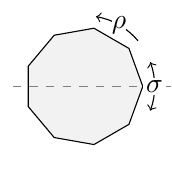
\begin{tikzpicture}[scale=0.75]
    \filldraw[fill=gray!10] (0:1) -- (40:1) -- (80:1) -- (120:1) -- (160:1) -- (200:1)-- (240:1)-- (280:1) -- (320:1) -- (0:1);
    \draw[dashed, gray, overlay] (-1.2,0) -- (1.5,0);
    \draw[<->, overlay] (20:1.2) arc[start angle=20, end angle=-20, radius=1.2] node[midway,fill=white,inner sep=1pt] {$\sigma$};
    \draw[<-, overlay] (80:1.2) arc[start angle=80, end angle=40, radius=1.2] node[midway,fill=white,inner sep=0] {$\rho$};
  \end{tikzpicture}
\end{wrapfigure}
Two famous examples of groups are the \emph{symmetric group}~$\Sym n$
of all permutations of the set $\Fin n \definedby \set{0, \dots,
n - 1}$, and the \emph{dihedral group}~$\Dih n$ of all
symmetries of a regular $n$-gon, i.e. $n$~rotations and
$n$~reflections. The dihedral group is \emph{generated} by a $2 \pi /
n$ rotation~$\rho$ and a single reflection~$\sigma$,
meaning every other symmetry can be obtained by a suitable composition
of $\rho$ and $\sigma$.\par\WFclear
\begin{wrapfigure}{r}*
  \newcommand{\twofortyeight}[1]{
    \begin{tikzpicture}[scale=0.4, tile/.style={rounded corners=0.05cm, minimum size=0.35cm, draw=white, thick, font=\sffamily}
      ]
      \foreach \x in {0,1,2,3} {
        \foreach \y in {0,1,2,3} {
          \node[tile, fill=gray!10] (\x\y) at (\x, \y) {};
        }
      }
      \foreach \row/\col/\num in {#1}
      \node[tile, fill=gray!10!orange!\num0] at (\col, 3 - \row) {};
      %%%%%%%%%%%%%%%%
      \draw[->,overlay] (4,2) arc[start angle=0, end angle=90, radius=2];
  \end{tikzpicture}}
  \twofortyeight{0/1/2, 0/3/2, 1/3/2, 2/1/2, 2/3/4, 3/1/4, 3/3/8}
\end{wrapfigure}%
\noindent{}%
In our examples, both the mirroring symmetry of trees and exchange of
colours are described by the symmetric group~$\Sym 2 =
\set{\stet,\swap}$, where $\stet$ is the identity permutation and
$\swap$ flips the two elements. The 2048 board is symmetric with
respect to the dihedral group~$\Dih 4$, though for our use, it is
sufficient to consider the \emph{cyclic group}~$\Cyc{4}$, generated by
the quarter-turn rotation marked here as~$\Rotation$.

\paragraph{Actions}

Groups capture symmetries abstractly. Symmetries between elements of a
particular set are captured by \emph{group actions}. Given a group
$\G$, recall that a \emph{$\G$-action} $\A = \seq*{\carrier A,
(\act)}$ consists of a \emph{carrier} set $\carrier \A$; and a map
$(\act) : \carrier \G \to \carrier \A \to \carrier \A$, writing
$(\act[\A])$ when ambiguous, such that:
\begin{itemize}
  \item every element is symmetric to itself via the neutral symmetry:
    $\unit \act x = x$ for $x \in \carrier\A$; and
  \item symmetry is transitive via composition:
    $(g_1 \mul g_2) \act x = g_1 \act (g_2 \act x)$ for
    $g_1, g_2 \in \carrier G$, $x \in \carrier A$.
\end{itemize}

\begin{example}
  \examplelabel{symmetric-group-action}
  The symmetric group $\Sym n$ acts on the finite sets $\Fin n = \set{0, 1,
    \dots, n - 1}$ by $\perm \act i \definedby \perm i$,
  and on vectors $\Vct n X \definedby X^n$ by
  \(
    \perm \act \seq{x_0, \dots, x_{n-1}} \definedby \seq{x_{\inv\perm 0}, \dots, x_{\inv\perm (n-1)}}
  \)
  sending the $i$-th element to the position  $\perm i$.
\end{example}

\begin{example}
  \examplelabel{2048 action}
  We define the sets of valid $n \times n$ boards of 2048 by:
  \[
    \Tile \definedby \set0\union \set{2^i \suchthat i \in \pnaturals}
    \qquad
    \Row n = \Vct n \Tile
    \qquad
    \Board n = \Vct n (\Row n)
  \]
  And the action $( \act ) : \Cyc 4 \to \Board n \to \Board n$ is
  given by rotating the board entries as:
  \[
    \Rotation \act
    \begin{psmallmatrix}
      x_{1,1} & \cdots & x_{1,n} \\
      \vdots & \ddots & \vdots \\[1ex]
      x_{n,1} & \cdots & x_{n,n}
    \end{psmallmatrix}
    =
    \begin{psmallmatrix}
      x_{1,n} & \cdots & x_{n,n} \\
      \vdots & \ddots & \vdots \\[1ex]
      x_{1,1} & \cdots & x_{n,1}
    \end{psmallmatrix}
  \]
  Since $\Rotation$ generates $\Cyc 4$, any other rotation is of the
  form $\Rotation^k$ for some $k$, and so the action of other
  rotations is uniquely determined by the group action laws to be
  ${\Rotation^k \act b = \Rotation \act (\Rotation^{k - 1} \act b)}$.

  Note, however, that not all definitions on generators extend to the
  whole group, as they must also respect the equalities between group
  elements. For example, since $\Rotation^4 = \unit$, we must also
  have that $\Rotation^4 \act b = b$ for any board~$b$, and the above
  definition respects that since rotating the entries four times gives
  us back the original matrix.
\end{example}

\paragraph{Equivariance}

The game 2048 exhibits symmetry not only by permitting rotations of
the board, but also by the fact that merging respects it: if we
rotate the board and then merge in the rotated direction, we get the
same result as first merging and then rotating the resulting board:
\[
  \newcommand{\twofortyeight}[2]{\vcenter{\hbox{
        \begin{tikzpicture}[scale=0.5, tile/.style={rounded corners=0.05cm, minimum size=0.45cm, draw=white, thick, font=\sffamily}
          ]
          \foreach \x in {0,1,2,3} {
            \foreach \y in {0,1,2,3} {
              \node[tile, fill=gray!10] (\x\y) at (\x, \y) {};
            }
          }
          \foreach \row/\col/\num in {#1}
          \node[tile, fill=gray!10!orange!\num0] at (\col, 3 - \row) {\small\num};
          %%%%%%%%%%%%%%%%
          #2
  \end{tikzpicture}}}}
  \begin{array}{ccccccc}
    \twofortyeight{0/1/2, 0/3/2, 1/3/2, 2/1/2, 2/3/4, 3/1/4, 3/3/8}
    {\draw[overlay, double distance=1.5pt
        , arrows = {-Latex[]}
    ]  (02.center) -- (01.center);}
    &\xmapsto{\Rotation}
    &\twofortyeight{2/0/2, 0/0/2, 0/1/2, 2/2/2, 0/2/4, 2/3/4, 0/3/8}
    {\draw[overlay, double distance=1.5pt
        , arrows = {-Latex[]}
    ]  (10.center) -- (20.center);}
    &\xmapsto{\Rotation}
    &\twofortyeight{3/2/2, 3/0/2, 2/0/2, 1/2/2, 1/0/4, 0/2/4, 0/0/8}
    {\draw[overlay, double distance=1.5pt
        , arrows = {-Latex[]}
    ]  (31.center) -- (32.center);}
    &\xmapsto{\Rotation}
    &\twofortyeight{1/3/2, 3/3/2, 3/2/2, 1/1/2, 3/1/4, 1/0/4, 3/0/8}
    {\draw[overlay, double distance=1.5pt
        , arrows = {-Latex[]}
    ]  (23.center) -- (13.center);}
    \\
    \downmapsto \scriptstyle\merge_{\Dn}
    &
    &\downmapsto \scriptstyle\merge_{\Rt}
    &
    &\downmapsto \scriptstyle\merge_{\Up}
    &
    &\downmapsto \scriptstyle\merge_{\Lt}
    \\
    \twofortyeight{1/3/4, 2/1/4, 2/3/4, 3/1/4, 3/3/8}{}
    &\xmapsto{\Rotation}
    &\twofortyeight{0/1/4, 2/2/4, 0/2/4, 2/3/4, 0/3/8}{}
    &\xmapsto{\Rotation}
    &\twofortyeight{2/0/4, 1/2/4, 1/0/4, 0/2/4, 0/0/8}{}
    &\xmapsto{\Rotation}
    &\twofortyeight{3/2/4, 1/1/4, 3/1/4, 1/0/4, 3/0/8}{}
  \end{array}
\]
\emph{Equivariance} captures symmetry preservation.
Given $\G$-actions $\A$ and $\B$, recall that an
\emph{equivariant} map
$\phi : \A \equito \B$
is a
map $\phi : \carrier
\A \to \carrier \B$ satisfying
\(
  \phi (g \act[\A] a) = g \act[\B] \phi a
\)
for all $g \in \carrier \G$ and $a \in \carrier \A$.

\begin{example}\examplelabel{action intro: permutation}
  Take any $f : X \to Y$. Its pointwise application
  $\vecmap f : \Vct n X \to \Vct n Y$
  is equivariant with respect to the permuting action of $\Sym n$ on
  vectors since:
  \begin{align*}
    \vecmap f (\perm \act \seq{x_0, \dots, x_{n-1}})
    &=
    \vecmap f (\seq{x_{\inv\perm 0}, \dots, x_{\inv\perm (n-1)}})
    =
    \seq{f x_{\inv\perm 0}, \dots, f x_{\inv\perm (n-1)}} \\
    &=
    \perm \act \seq{f x_0, \dots, f x_{n-1}}
    =
    \perm \act (\vecmap f \seq{x_0, \dots, x_{n-1}})
    \tag*{\qedhere}
  \end{align*}
\end{example}

Before the next example, recall that a \emph{product} $\A \times \B$
of $\G$-actions $\A$ and $\B$ is given on
\(
  \carrier{\A \times \B} \definedby {\carrier \A} \times {\carrier \B}
\)
component-wise by:
\(
  g \act[\A \times \B] \seq{a, b} \definedby \seq{g \act[\A] a, g \act[\B] b}
\).
Furthermore, the \emph{exponential action} $\A \to \B$ is given on
the set of all functions, not only the equivariant ones,
\(
  \carrier{\A \to \B}\definedby \carrier\A \to \carrier\B
\)
by \emph{conjugation}:
\(
  (g \act[\A \to \B] f) \definedby \fun a g \act[\B]  f(\inv g\act[\A] a)
\).
Finally, the \emph{trivial} action $\Triv \X$ on a set $\X$ is defined by
\(
  \carrier{\Triv \X} \definedby \X
\) and \(
  g \act x \definedby x \). An \emph{invariant} map is an equivariant
map $f : \A \equito \Triv \X$.

\begin{example}
  \examplelabel{tree example}
  We can equip the set $\Tree$ of binary trees with values in
  $\naturals$ (fixed for simplicity) with the recursive $\Sym2$-action
  $\swap \act[\Tree] {\Leaf} = \Leaf$ and ${\swap} \act[\Tree] \Node(\ell, n, r) =
  \Node(\swap \act r,n,\swap \act \ell)$. Furthermore, let $\TreePath$
  be the set of lists over step directions $\TreeLabel = \set{\Lft,\Rgt}$. We can
  equip $\TreePath$ with an $\Sym2$-action by mapping the
  $\Sym2$-action $\swap \act \Lft = \Rgt$ and $\swap \act \Rgt = \Lft$.

  Take $\lookup : \Tree \to \TreePath \to \Maybe\naturals$, which
  takes a path through a tree (a list of steps left or right) and
  returns the resulting value, if it exists. This function is
  invariant under symmetry: if we flip both the tree and the direction
  of all the steps, we should get back the same value. More precisely,
  $\lookup$ is equivariant in its curried form $\Tree \equito
  (\TreePath \to \Triv(\Maybe\naturals))$ with respect to the
  exponential action, while the uncurried form $\Tree \times \TreePath
  \equito \Triv(\Maybe\naturals)$ is invariant.
\end{example}

\subsection{The \WLOG construction}
\subseclabel{wlog-construction}

\paragraph{Canonisers}

The first step in our construction is to map each input to a
\emph{canonical} representative.  Crucially, we canonise via
an explicit symmetry in the group, rather than through an arbitrary
function, as we need to apply the inverse symmetry to reconstruct the
output for the original input.

For example, we canonise search trees by flipping the tree when the
inserted key is strictly larger than the root key. Thus, the remaining
canonical inputs are those that: insert into an empty tree, insert the
redundant key equal to the one in the root; and insert to the left
subtree. For the pigeonhole principle example, the canonising symmetry
is the identity if the first object is red, and $\swap$ that exchanges
the colours if the first object is blue. Thus, the canonical elements
are triples in which the first object is red.

\begin{definition}
  Let $\A$ be a $\G$-action. A \emph{canoniser} for $\A$ is a function
  $\canoniser : \carrier A \to \carrier G$. For each $a \in \carrier
  A$, we call the symmetry $\canoniser a \in \carrier G$ the
  \emph{$\canoniser$-canonising symmetry} of $a$, and the element
  $\canoniser a \act a \in \carrier A$ the \emph{canonical form}
  of $a$.
  We define the set of \emph{canonical} elements to be
  \(
    \Canon[\A]\canoniser \definedby \set*{\canoniser a \act a
    \suchthat* a \in \carrier \A}
  \).
\end{definition}

Canonisers need not respect the structure of the
action on $A$, as many of the interesting examples indeed do not.
However, there are still some examples that respect it, and we study
them and their impact on the equivariance of the \WLOG{} construction
in \subsecref{wlog-equivariance}.

\begin{example}
  \examplelabel{sorting canoniser}
  Let $P$ be a \emph{strict partial order}, i.e., a set equipped with
  an irreflexive and transitive relation~$<_P$. We say that an
  $n$-tuple $\vec p \in \Vct n P$ is \emph{sorted} when $p_{i} <
  p_{j}$ implies $i < j$ for all indices $i, j \in \Fin n$. Then, a
  \emph{sorting function} is a function $\sort : \Vct n P \to
  \carrier{\Sym n}$ that maps a tuple to a permutation that sorts it.
  Every such function is a canoniser for the permuting action of $\Sym
  n$ on $\Vct n P$ from \exampleref{symmetric-group-action}.

  Given an $n$-tuple $\vec p$, the sorted tuple $(\sort \vec p) \act
  \vec p$ is the canonical form of $\vec p$, and every $p \in \Canon\sort$
  is sorted. If the sorting function returns the identity
  permutation for sorted tuples---for example when the sorting is
  stable---the set $\Canon\sort$ is exactly the set of sorted tuples.
\end{example}

\begin{example}
  \examplelabel{2048 canoniser}
  Continuing \exampleref{2048 action}, the input for the 2048's merge
  is the board together with the merge direction. Define $\Direction
  \definedby \set{\Rt, \Up, \Lt, \Dn}$ and its action $(\act) : \Cyc 4
  \to \Direction \to \Direction$ by:
  \[
    \Rotation \act \Rt \definedby \Up
    \quad
    \Rotation \act \Up \definedby \Lt
    \quad
    \Rotation \act \Lt \definedby \Dn
    \quad
    \Rotation \act \Dn \definedby \Rt
  \]
  Define $\mkLt[] : \Direction \to \carrier{\Cyc 4}$ to pick the
  unique rotation turning its input left, i.e. $(\mkLt d) \act d = \Lt
  $:
  \[
    \mkLt \Rt \definedby \Rotation^2 = \twiceRotation
    \qquad
    \mkLt \Up \definedby \Rotation
    \qquad
    \mkLt \Lt \definedby \unit = \nonRotation
    \qquad
    \mkLt \Dn \definedby \inv\Rotation = \unRotation
  \]
  Thus the only canonical direction is left
  $\Canon{\mkLt[]} = \set{\Lt}$. We can extend the
  canoniser to input pairs $\Direction \times \Board n$ by
  $\mkLt \compose \projection_1$.
\end{example}

We frequently encounter similar canonisers that depend only on a part of the
input.

\begin{lemma}\lemmalabel{projection canoniser}
  Let $\A$ and $\B$ be $\G$-actions. Every $\A$-canoniser $\canoniser
  : \carrier\A \to \carrier\G$ induces an
  $(\A\times\B)$-canoniser $\canoniser \compose \projection_1 :
  \carrier {\A \times\B} \to \carrier \G$. We then have
  $\Canon{\parent{\canoniser \compose \projection_1}} =
  \Canon\canoniser \times \carrier\B$.
\end{lemma}

\paragraph{Core functions}

Given $\G$-actions $\A$ and $\B$, we want to define a
function $\A \to \B$ while avoiding symmetric cases. Once we have an
$\A$-canoniser~$\canoniser$ and its set of canonical
elements~$\Canon\canoniser$ in place, the only thing missing is the
\emph{core function} $f : \Canon\canoniser \to \carrier\B$:
merging of tiles in 2048, insertion into
a subtree, or the special case in the pigeonhole principle.
Typical symmetric \WLOG arguments only explicate canonical elements and core functions,
but gloss over groups, actions, and canonisers.

\begin{example}
  \examplelabel{2048 core function}
  Continuing \exampleref{2048 canoniser}, let us define the core
  function merging the tiles in 2048. We choose left merges as the
  canonical direction since vertical merges go against the structure
  of vectors of rows, while rightward merges have edge cases
  coalescing empty tiles. First, we define $\mergeLeft[\Row{}] : \Row
  n \to \Row n$ using pattern matching as all the relevant tiles are
  on the left:
  \begin{gather*}
    \mergeLeft[\Row{0}] \seq{}
    \definedby \seq{}
    \quad
    \mergeLeft[\Row{1}] (x :: \seq{})
    \definedby \seq{x}
    \quad
    \mergeLeft[\Row{1+n}] (0 :: r)
    \definedby \mergeLeft[\Row{n}](r) \++ \seq{0}
    \\
    \mergeLeft[\Row{2+n}] (x :: y :: r)
    \definedby
    \begin{cases}
      2 x :: \mergeLeft[\Row{n}](r) \++ \seq{0} & (x = y) \\
      \mergeLeft[\Row{1+n}](x :: r) \++ \seq{0} & (y = 0) \\
      x :: \mergeLeft[\Row{1+n}](y :: r) & (x \ne y \ne 0)
    \end{cases}
  \end{gather*}
  We merge the whole board simply by merging each row:
  \[
    \mergeLeft : \Board n \to \Board n
    \qquad
    \mergeLeft \definedby \vecmap \mergeLeft[\Row{n}]
    \tag*{\qedhere}
  \]
\end{example}

\paragraph{The construction}

We now formally define the \WLOG{} construction we sketched a number of
times, extending a core function $f : \Canon\canoniser \to \carrier
\B$ to the whole carrier $\carrier\A$.  Take any $a \in \carrier\A$
and compute its canonical form $\canoniser a \act a$. By
definition, the canonical form lies in $\Canon\canoniser$, so we can
apply the core function to obtain $f (\canoniser a \act a)$. Even
though this result has the expected type~$\B$, we still need to apply
the inverse symmetry $\ginv*{\canoniser a}$.
Indeed, making a downward merge in 2048 would result in a
rotation, followed by a leftward merge, followed by the inverse rotation.

\begin{definition}
  Let $\A$ and $\B$ be $\G$-actions, $\canoniser : \carrier\A \to
  \carrier\G$ a canoniser, and $f : \Canon\canoniser \to \carrier\B$
  a core function. Then, the \emph{\WLOG construction}~$\wlg(c,f) :
  \carrier\A \to \carrier\B$ is defined as
  \[
  \myfigbox{$
    \wlg(\canoniser,f) \definedby
    \fun{a} \ginv*{\canoniser a}\act[\B] f(\canoniser a \act[\A] a)
  $}
  \]
\end{definition}
%
Using \exampleref{2048 core function}, we define $\merge : \Direction \times \Board n
\to \Board n$ as $\wlg(\mkLt \compose \projection_1, \mergeLeft \compose \projection_2)$.

\subsection{Equivariance of the \WLOG construction}
\subseclabel{wlog-equivariance}

In addition to extending the core function $f : \Canon\canoniser \to
\carrier\B$ to the whole domain, we often want the extension $\phi :
\carrier\A \to \carrier\B$ to be equivariant. This requirement implies that the
core function $f$ must already behave equivariantly where defined. To
see this, consider a canonical element $x \in \Canon\canoniser$ that
also has a symmetric canonical element $g \act x \in
\Canon\canoniser$. Then:
\[
\myfigbox{
  $
  f(g \act x)
  \explain={$\phi$ extends $f$}
  \phi(g \act x)
  \explain={$\phi$ is equivariant}
  g \act \phi(x)
  \explain={$\phi$ extends $f$}
  g \act f x
  $}
\]
We generalise the notion of equivariance to domains that may
not be closed under the action:

\begin{definition}
  Take $\G$-actions $\A$, $\B$, a subset $X \subseteq \carrier\A$,
  and a function $f : X \to \carrier\B$. We call $f$ \emph{equivariant},
  writing $f : (X \subseteq A)
  \equito \B$, when
  \(
    g \act x \in X \implies f (g \act x) = g \act f x
  \)
  for $g \in \carrier\G$, $x \in X$.
\end{definition}

\begin{example}
  Every core function for the 2048 canoniser from \exampleref{2048
  canoniser} is vacuously equivariant: only $\Lt$ is
  canonical, and any $g \in \Cyc{4}\setminus\set\unit$ changes the
  direction to a non-canonical input. Therefore, if $x, g \act x$ are
  canonical, then $g = \unit$ and $g \act f\,x = f\,x = f(g \act x)$.

  Insertion into binary search trees features non-trivial corner cases
  of core function equivariance. Flipping the empty tree yields back the
  empty tree, which is again a canonical element. Thus inserting a key
  into a ``flipped'' empty tree needs to be the same as first inserting
  the key into the empty tree and then flipping the result. However, the
  resulting tree is a single root with two empty subtrees, which is
  invariant under flipping, thus the core function is equivariant.
  A similar case occurs when inserting a key that is equal to the root value.
\end{example}

Equivariance of core functions is easily overlooked when canonical
elements are treated in isolation, especially since the overlap
usually occurs on trivial cases. On a more positive note, the
condition is not only necessary, but also sufficient for the existence
of an equivariant extension. Furthermore, \WLOG{} gives the unique
such extension:

\begin{theorem}
  \theoremlabel{wlog-construction}
  Let $\A$ and $\B$ be $\G$-actions and $\canoniser : \carrier\A \to
  \carrier\G$ a canoniser. If $f : (\Canon\canoniser \subseteq \A)
  \equito \B$ is an equivariant core function, then $\wlg(c,f) : \A
  \equito \B$ is the unique equivariant function extending $f$ to the
  whole $\carrier\A$, along the inclusion $\Canon\canoniser \subset \carrier\A$.
\end{theorem}

\begin{example}
  Recall the $2048$ function
  $\merge = \wlg(\mkLt, \mergeLeft) : \Direction \times \Board n \to
  \Board n$.
  It indeed behaves as expected: for leftward merges, it
  extends $\mergeLeft$, while for other directions, it is uniquely
  determined by the equivariant behaviour.
\end{example}

In concrete cases, equivariance of core functions is often easily
discharged, but we can further relax it when the
canoniser~$\canoniser$ has additional properties. A natural property
is the equivariance of the canoniser. Since $\parent{\canoniser a \mul
\inv g} \act (g \act a) = \canoniser a \act a$ is canonical, it is
natural to ask whether $\canoniser a \mul \inv g$ is the
$\canoniser$-canonising symmetry of $g \act a$, i.e. whether
$\canoniser(g \act a) = \canoniser a \mul \inv g$. More succinctly,
this property means $\canoniser$ is an equivariant map $\canoniser :
\A \equito \inv\G$ where $\inv\G$ is the action of $\G$ on itself,
defined by $g \act[\inv\G] h \definedby h \mul \inv g$. It validates
the axioms since:
%
\begin{gather*}
  \unit \act[\inv\G] s = s \mul \inv\unit = s
  \qquad
  g \act[\inv\G] (h \act[\inv\G] s)
  =
  (s \mul \inv h)\mul \inv g = s \mul \inv*{g \mul h} = (g \mul h)\act[\inv\G] s
\end{gather*}

\begin{definition}
  A canoniser $\canoniser : \carrier\A \to \carrier\G$ is
  \emph{strictly equivariant} when $\canoniser\parent{g \act a} =
  \canoniser a \mul \inv g$, i.e. when it is an equivariant map
  $\canoniser : \A \equito \inv\G$.
\end{definition}

As we shall soon see, strict equivariance is a powerful assumption,
but also a very strong restriction, thus we reserve the name
\emph{equivariant canonisers} for a weaker and more natural
notion that we introduce in \subsecref{equivariant canonisers}, after
we discuss dependent types.

\begin{example}
  \examplelabel{strictly equivariant canonisers}
  The canoniser $\mkLt[]$ from \exampleref{2048 canoniser} is strictly
  equivariant since $\mkLt d$ is the unique rotation that makes $d$
  canonical. On the other hand, if in \exampleref{sorting canoniser},
  we take a non-total ordering $\P$ and a stable sorting algorithm,
  the canoniser $\sort : \Vct n P \to \carrier{\Sym n}$ is not
  strictly equivariant since for every two incomparable elements $p, q$,
  we have:
  \begin{align*}
    \mspace{-10mu}\sort\parent{(0 \leftrightarrow 1)\act \seq{p,q}}
    &= \sort\seq{q,p} = \id
    \neq (0 \leftrightarrow 1) = \id \mul \inv{(0 \leftrightarrow 1)} = (0 \leftrightarrow 1) \act \sort\seq{p,q}
    \mspace{-10mu}
    \tag*{\qedhere}
  \end{align*}
\end{example}

Strict equivariance guarantees equivariance of arbitrary core functions,
and thus also of the \WLOG{} construction. The converse also holds,
though we do not need it for our applications.

\begin{theorem}
  \theoremlabel{all core functions are partially equivariant}
  Let $c : \carrier\A \to \carrier\G$ be a canoniser. Then,
  $\canoniser$ is strictly equivariant iff for every action $\B$,
  every core function $f : \Canon\canoniser \to \carrier\B$ is
  equivariant.
\end{theorem}

Strict equivariance is too strong, as it restricts the action to
be \emph{semi-regular}, meaning that only the identity can fix an
element: $g \act a = a \implies g = \unit$.

\begin{lemma}[semi-regularity]\lemmalabel{semi-regularity}
  If $\A$ has a strictly equivariant canoniser, then $\A$ is
  semi-regular.
\end{lemma}

For example, the $\Cyc 4$ action on $\Board n$ is not semi-regular,
since all rotations preserve the empty 2048 board. It is only the
addition of the direction, which all non-trivial symmetries affect,
that makes the action on $\Direction \times \Board n$ semi-regular.

Strictly equivariant canonisers satisfy $\canoniser(\canoniser a
\act a) = \canoniser a \mul \inv*{\canoniser a} = \unit$, meaning that
canonisation is a one-step process and that further canonisation
symmetries are identities. This observation leads us to a weaker natural property
of canonisers, and one that all examples in this paper enjoy:

\begin{definition}
  A canoniser $\canoniser$ is \emph{immediate} when for all $a \in
  \carrier\A$, we have $\canoniser(\canoniser a \act a) = \unit$.
\end{definition}

\begin{proposition}\propositionlabel{strictly equivariant canonisers are immediate}
  A strictly equivariant canoniser $\canoniser : \A \equito \inv\G$ is immediate.
\end{proposition}

The converse does not hold: as we saw in \exampleref{strictly
equivariant canonisers}, a stable sorting function is not a strictly
equivariant canoniser, but it is immediate since the canonical
elements are exactly the sorted tuples, and the sorting permutation
for sorted tuples is the identity.

We will often derive a canoniser for $\A\times\B$ from a canoniser for
$\A$ through projection. For example, we
derive the canoniser for $\Direction\times\Board{n}$ from that of $\Direction$.

\begin{lemma}\lemmalabel{equivariance of projection canonisers}
  For $G$-actions $\A, \B$, if $\carrier \A \xto{\canoniser} \carrier
  \G$ is strictly equivariant/immediate, then so is
  $\carrier \A \times \carrier \B \xto{\canoniser
  \compose \projection_1} \carrier
  \G$.
\end{lemma}

To apply the \WLOG construction, we need to provide both the
canoniser~$\canoniser$ and the core function~$f$. If we have
$\canoniser a = \unit$ for some $a \in \carrier\A$, then $a =
\canoniser a \act a \in \Canon\canoniser$, and so we need to define
the value $f a$. In the ideal case, we want to consider each element
of $\carrier\A$ only once and define the core function only on
elements with trivial canonising symmetries. More precisely, we want
the sets $\set{a \in \carrier A \suchthat \canoniser a \ne \unit}$ and
$\Canon\canoniser$ to be disjoint. But in general, the two sets may
overlap. In the extreme case, if
\(
  \canoniser : \Direction \to \carrier{\Cyc4}
\)
is the constant function
\(
  \fun{\_} \Rotation
\),
they are both equal to the whole domain $\Direction$. However,
immediate canonisers are exactly those for which the domain
$\carrier\A$ cleanly splits into two:

\begin{proposition}
  \propositionlabel{immediate canonical is kernel}
  A canoniser $\canoniser : \carrier\A \to \carrier\G$ is immediate
  iff $\Canon\canoniser = \inv{\canoniser}[\unit] \definedby \set{a
  \in \carrier A \suchthat \canoniser a = \unit}$.
\end{proposition}
